\documentclass[11pt]{article}
\usepackage{latexsym}
\usepackage{amsmath}
\usepackage{amssymb}
\usepackage{amsthm}
\usepackage{epsfig}
\usepackage[tight]{subfigure}
\usepackage{bm}

\usepackage{amsmath}

\DeclareMathOperator*{\minimize}{min}
\DeclareMathOperator*{\maximize}{max}

\usepackage{algorithm}
 %on linux you may need to run sudo apt-get install texlive-full to install algorithm.sys
\usepackage{algorithmic}

\usepackage{verbatim}

\newcommand{\handout}[5]{
  \noindent
  \begin{center}
  \framebox{
    \vbox{
      \hbox to 5.78in { {#1} \hfill #2 }
      \vspace{4mm}
      \hbox to 5.78in { {\Large \hfill #5  \hfill} }
      \vspace{2mm}
      \hbox to 5.78in { {\em #3 \hfill #4} }
    }
  }
  \end{center}
  \vspace*{4mm}
}

\newcommand{\lecture}[5]{\handout{#1}{#2}{#3}{#4}{#5}}
\newcommand{\collision}[0]{\mathrm{collision}}
\newcommand{\nocollision}[0]{\overline{\collision}}

\newcommand*{\QED}{\hfill\ensuremath{\square}}

\newcommand{\argmax}[1]{\underset{#1}{\operatorname{arg}\,\operatorname{max}}\;}
\newcommand{\argmin}[1]{\underset{#1}{\operatorname{arg}\,\operatorname{min}}\;}

\newtheorem{theorem}{Theorem}
\newtheorem{corollary}[theorem]{Corollary}
\newtheorem{lemma}[theorem]{Lemma}
\newtheorem{observation}[theorem]{Observation}
\newtheorem{proposition}[theorem]{Proposition}
\newtheorem{definition}[theorem]{Definition}
\newtheorem{claim}[theorem]{Claim}
\newtheorem{fact}[theorem]{Fact}
\newtheorem{assumption}[theorem]{Assumption}
\newtheorem{note}[theorem]{Note}

% 1-inch margins, from fullpage.sty by H.Partl, Version 2, Dec. 15, 1988.
\topmargin 0pt
\advance \topmargin by -\headheight
\advance \topmargin by -\headsep
\textheight 8.9in
\oddsidemargin 0pt
\evensidemargin \oddsidemargin
\marginparwidth 0.5in
\textwidth 6.5in

\parindent 0in
\parskip 1.5ex
%\renewcommand{\baselinestretch}{1.25}

\begin{document}

\lecture{Statistical Techniques in Robotics (16-831, S21)}{Lecture \#09
  (Wednesday, March 3)}{Lecturer: Kris Kitani}{Scribes: Andy Wei, Yi-Chun Chen}{OGD \& NormExpGD}

\section{Review}
In the last lecture, we talked about online mirror descent (OMD). In this section, we will first give the review of OMD, dive into the definitions of Conjugate Function and Bregman Divergence, and finally lead to the analysis of OMD.
\vspace{-3mm}
\subsection{Online Mirror Descent}
Online mirror descent is formulated from follow the regularized leader (FTRL)\cite{mcmahan2011follow}. 
%Algorithm \ref{algo:ftrl} shows the algorithm of FTRL with linear loss. 
By reparametrizing as dual parameter %(see Equation \ref{eq:dual_param}) 
and mirror function %(see Equation \ref{eq:mirror_fn})
, when FTRL loss is linear, and regularization is convex, it is named as OMD. The idea is to optimize in the dual space and mirror in the primal space, as shown in Algorithm \ref{algo:omd}.

% \begin{algorithm}[H]
% \caption{FTRL-LINLOSS (Convex set \emph{S})}
% \label{algo:ftrl}
% \begin{algorithmic}[1]

% \FOR{$t=1,\;\cdots,\;T$}
% \STATE $\bm{w}^{(t)}$ = $\argmin{\bm{w}} \sum_{i=1}^{t-1} \big \langle \bm{w},\bm{z}^{(i)}\big \rangle + \psi(\bm{w}) $\hfill
% \STATE $\textsc{Receive} (f^{(t)}: S\rightarrow \mathbb{R})$\hfill
% \ENDFOR
% \end{algorithmic}
% \end{algorithm}

% \begin{equation}
% \label{eq:dual_param}
%     \bm{\theta}^{(t+1)} \triangleq -\bm{z}^{(1:t)}
% \end{equation}
% \begin{equation}
% \label{eq:mirror_fn}
%     g(\bm{\theta}^{(t+1)}) \triangleq \argmax{\bm{w}} \big \langle \bm{w}, \bm{\theta}^{(t+1)} \big \rangle - \psi(\bm{w})
% \end{equation}


\begin{algorithm}[H]
\caption{OMD (Convex set \emph{S}, \emph{g}: $\mathbb{R}^\emph{D} \rightarrow \emph{S})$}
\label{algo:omd}
\begin{algorithmic}[1]

\FOR{$t=1,\;\cdots,\;T$}
\STATE $\textsc{Receive} (f^{(t)}: S\rightarrow \mathbb{R})$\hfill $\triangleright$ $f^{(t)}(\cdot)$: time-varying loss function
\STATE $\bm{\theta}^{(t+1)}$ = $\bm{\theta}^{(t)} - \eta\bm{z}^{(t)}, \bm{z}^{(t)} \in \partial f^{(t)}(\bm{w}^{(t)})$ \hfill  $\triangleright$ \bm{$\theta$}: parameters in dual space
\STATE $\bm{w}^{(t+1)}$ = $\emph{g}(\bm{\theta}^{(t+1)})$\hfill $\triangleright$  $g(\cdot)$: mirror function

\ENDFOR
\end{algorithmic}
\end{algorithm}
\vspace{-3mm}
\subsection{Conjugate Function}
\subsubsection{Primal Representation and Dual Representation}
First we need to know parametrizations of a function in primal space and dual space:
$$
    Primal: \{\psi(\emph{w}),\; \emph{w}\} \;\;\;\;\;  Dual: \{\emph{b}(\emph{$\theta$}),\; \emph{$\theta$}\}
$$
, where \emph{w} and $\psi$(\emph{w}) are the parameter and function and \emph{$\theta$} and \emph{b}(\emph{$\theta$}) are the slope and intercept. Then, let's look into the dual parametrization in dual space in the aspect of geometry.

\begin{figure}
    \centering
    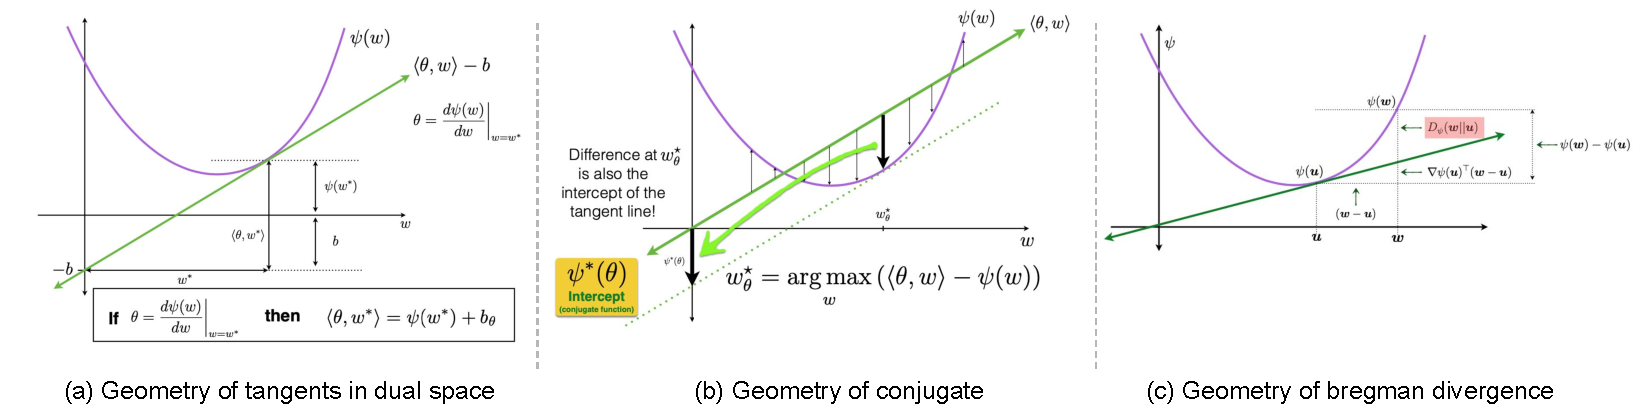
\includegraphics[width=1.\textwidth]{images/review.pdf}
    \caption{Geometry representation for review section.}
    \label{fig:review}
\end{figure}

In Figure \ref{fig:review} (a), we observe that when $\theta$ = $\left.\frac{d\psi(w)}{dw}\right|_{w=w^*}$ holds, \big \langle $\theta$, $w^*$ \big \rangle = $\psi(w^*) + b_\theta$. For a corresponding pair $\{\theta, w^*\}$, we rearrange the equation above and have
$$
-b(\theta) = - \big \langle \theta, w^*(\theta) \big \rangle + \psi(w^*(\theta))
$$

\subsubsection{Geometry of Conjugate Function}
In Figure \ref{fig:review} (b), consider a function $\big \langle \theta, w \big \rangle - \psi(w)$, we can observe we can find a $w_\theta^*$ that maximizes the function. Also, at $w_\theta^*$, the difference of the functions is also the intercept of the tangent line, $\psi^*(\theta)$. It is concluded that the conjugate function is, for any slope $\theta$, $\psi^*(\theta)$ = $\max_{w}(\big \langle \theta, w \big \rangle - \psi(w))$.

% \subsubsection{Properties of Convex Conjugate}
% % \noindent Definition of the convex conjugate: $\psi^*(\bm{\theta})$ = $\max_{\bm{w}}(\big \langle \bm{\theta}, \bm{w} \big \rangle - \psi(\bm{w}))$

% \noindent Derivative of the convex conjugate: $\nabla_\theta\psi^*(\bm{\theta})$ = $\frac{\partial\psi^*(\bm{\theta})}{\partial\bm{\theta}} = \bm{w}^*$ \;\; $\nabla_w\psi^*(\bm{w})$ = $\left.\frac{\partial\psi(\bm{w})}{\partial \bm{w}}\right|_{w=w^*}$ = $\bm{\theta}$

% \noindent Derivative of the convex conjugate: $\nabla_\theta\psi^*(\bm{\theta})$ = $\argmax{w}(\big \langle \bm{\theta}, \bm{w} \big \rangle - \psi(\bm{w}))$

% \noindent Fenchel-Young Inequality: 
% $\psi^*(\bm{\theta}) \geq (\big \langle \bm{w}, \bm{\theta} \big \rangle - \psi(\bm{w}))$ 
% \vspace{-3mm}

\subsection{Bregman Divergence}
The definition of Bregman Divergence is below; that is, the distance between two points according to some proximity function $\psi$, which in the context of OMD is the regularization function. Geometrically, as show in Figure \ref{fig:review}, (c) it is the approximation error between a linear approximation of some convex function.
$$
    \bm{D}_\psi(\bm{w}||\bm{u}) = \psi(\bm{w}) - \psi(\bm{u}) - \nabla\psi(\bm{u})^T(\bm{w} - \bm{u})
$$

\vspace{-3mm}
\subsection{OMD Analysis}
We aim to analyze the regret bound of OMD. The loss of any arbitrary vector $\bm{u}$ is
$$
\psi(\bm{u}) + \sum_{t=1}^T \bm{u} \cdot \bm{z}^{(t)} = \psi(\bm{u}) - \bm{u} \cdot \bm{\theta}^{(T+1)}
$$
By applying Fenchel-Young Inequality $\psi^*(\bm{\theta}) \geq (\big \langle \bm{w}, \bm{\theta} \big \rangle - \psi(\bm{w}))$ to RHS, we get
$$
\psi(\bm{u}) - \bm{u} \cdot \bm{\theta}^{(T+1)} \geq -\psi^*(\bm{\theta^{(T+1)}})
$$

Next, expand the RHS with telescoping and we can derive the general OMD regret bound as follow:
$$
R(\bm{u}) = \sum_{t=1}^T \bm{w}^{(t)} \cdot \bm{z}^{(t)} - \bm{u} \cdot \bm{z}^{(t)}
\leq \psi(\bm{u}) - \psi(\bm{w}^{(1)}) + \sum_{t=1}^{T} D_{\psi^*}(-\bm{z}^{(1:t)} || -\bm{z}^{(1:t-1)})
$$

% OMD
% Duality- Convex Conjugate, Bregman Divergence
% Conjugate Function - convex conjugate, Fenchel dual, Fenchel conjugate, Fenchel transform
% Fenchel-Young Inequality
% General OMD regret bound
% different regularization functions leads to different algorithm -> OGD


% In this lecture, we will talk about OGD, OMD with a linear loss and quadratic regularization.

% This section serves as a review of the previous lecture and any other context required to frame the content of the current lecture. 

% You may format the scribes in any way you like, aside from changing font style, size and page format. Please use subsections and paragraphs to increase the readability of your notes.

%Length requirement 1-2 pages.
        

% We recall the characteristics of the problem of Prediction with Expert Advice \cite{littman2015reinforcement} (an online learning problem):
% \begin{enumerate}
%     \item One-Shot: The data arrives as a stream, but its sequence is not correlated.
%     \item Instructive: We receive a fully observable loss based on the prediction made.
%     \item Exhaustive: We will eventually have access to the entire state and action space.
% \end{enumerate}
% Clearly, the key distinction from supervised learning setting arises from the fact that there is no distinct train and test stage, and input \& output are given in sequence. This distinction also leads to a different kind of analysis, in terms of bounds on mistakes and regrets, as we will develop later.

% \subsection{Realizability}

% \definition{\normalfont\textbf{Realizability} is the assumption that the learner has access to the perfect hypothesis.}

% \normalfont
% To discuss further, we recall that under the conditions of realizability, the performance is measured in terms of the mistake bound, which represents, in retrospect, the cost for not following the perfect hypothesis. Under this assumption of realizability, previously we had seen the halving (Majority) algorithm, which maintains a set of hypothesis (the version space) consistent with past evidence, i.e. it predicts according to the majority vote of hypothesis from the version space. We had also obtained the mistake bound of the halving algorithm to be logarithmic in the number of hypotheses, since it removes at least half the hypotheses after one mistake. 

% However, we will now relax this realizability assumption and allow even the best expert to make a few mistakes. Under these new conditions of non-realizability, we will evaluate the performance of the algorithm in terms of the \textit{regret bound} instead of the \textit{mistake bound}. In such a case, we would like to design algorithms demonstrating small regrets. Accordingly, we start with providing the (mathematical) definition of regret below.
% \definition{\normalfont\textbf{Regret} of the learner, $R^{(T)}(H)$, is the cumulative loss for not following the best hypothesis in the hypothesis class $H$. Regret can be mathematically formulated as follows:}
% \begin{align}
%     R^{(T)}(H)=\sum_{t=1}^{T} l(\hat{y}^{(t)}, y^{(t)}) - \minimize_{h\in H}  \sum_{t=1}^{T} l(h(x^{(t)}), y^{(t)})\label{def:regret}
% \end{align}
% \normalfont
% where, $\sum_{t=1}^{T} l(\hat{y}^{(t)}, y^{(t)})$ represents the cumulative loss of the learner, and $\minimize\sum_{t=1}^{T} l(h(x^{(t)}), y^{(t)})$ represents the loss of best single hypothesis. 

% Clearly, the regret bound is a more general performance bound, of which the mistake bound is a special case. In this lecture, we will use the regret bound to characterize online algorithms and conversely, we will be interested in finding good algorithms as characterized by this regret bound. We recall that in previous lectures, we had assumed at least one perfect algorithm, which implies realizability. However, in this lecture, the first algorithm we will consider is under the relaxed assumption of non-realizability, namely, the Weighted Majority Algorithm (WMA), which has a multiplicative weighting on the experts that decays with the number of mistakes.

% \definition{\normalfont\textbf{Potential Function} is the sum of the weights, a non-integer scalar equivalent to the size of the version space, used in the context of Weighted Majority algorithms.}

\section{Summary}
\subsection{Online Gradient Descent (OGD)}
\subsubsection{Gradient Descent}
\normalfont
Gradient descent \cite{gd1847} is the standard approach for minimizing differentiable convex functions. The gradient descent is listed as Algorithm \ref{algo:gd} below. The line 4 specifies that the algorithm updates weight by gradient with a scaling factor $\eta$. The gradient, denoted a $\nabla f(\textbf{w})$ in the line 3, is a gradient of a differentiable function $f: \mathbb{R}^N \rightarrow \mathbb{R}$ at $\textbf{w}$. It is a vector of a parital derivatives

$$\nabla f(\text{w}) = \{ \frac{\partial f(\textbf{w})}{\partial w_1},  \frac{\partial f(\textbf{w})}{\partial w_2}, \cdots, \frac{\partial f(\textbf{w})}{\partial w_N} \}$$



\begin{algorithm}[H]
\caption{Gradient Descent (GD)}
\label{algo:gd}
\begin{algorithmic}[1]
\STATE $\textbf{w}^{(0)} \leftarrow 0$ \hfill $\triangleright$ Weight initialization

\FOR{$t=1,\;\cdots,\;T$}
\STATE \textsc{Compute} ($\nabla f(\textbf{w}^{(t-1)})$) \hfill $\triangleright$ Compute gradient of current step w.r.t. weight
\STATE $\textbf{w}^{(t)} = \textbf{w}^{(t-1)} - \eta \nabla f(\textbf{w}^{(t-1)})$ \hfill $\triangleright$ Update weight by gradient and learning rate $\eta$
\ENDFOR
\end{algorithmic}
\end{algorithm}

\subsubsection{Understanding Gradient Descent}
One may ask how the update equation comes from. There are 3 perspectives of viewing GD algorithm: geometric, linear approximation with regularization, and isometric quadratic approximation. \\
\textbf{Geometric   }
The first, most intuitive way is - moving in the direction opposite of the gradient. It is easy to say that when the learning rate is sufficiently small, we could minimize the function value by moving in such direction. However, such perspective is not very rigorous.\\
\textbf{Linear Approximation with Regularization   }
The second perspective comes from linear approximation. Given $\textbf{w}$, we can approximate the $f(\textbf{u})$ by first-order Taylor expansion.
$$f(\textbf{u}) \approx f(\textbf{w}) + \langle (\textbf{u} - \textbf{w}), \nabla f(\textbf{w}) \rangle$$

Our objective of minimizing function value f will then become
$$\min_u f(\textbf{u}) \approx \min_u \{f(\textbf{w}) + \langle (\textbf{u} - \textbf{w}), \nabla f(\textbf{w}) \rangle\}$$
However, directly minimize the above equation will lead to solution at negative infinity.
\begin{center}
    \hspace{3cm}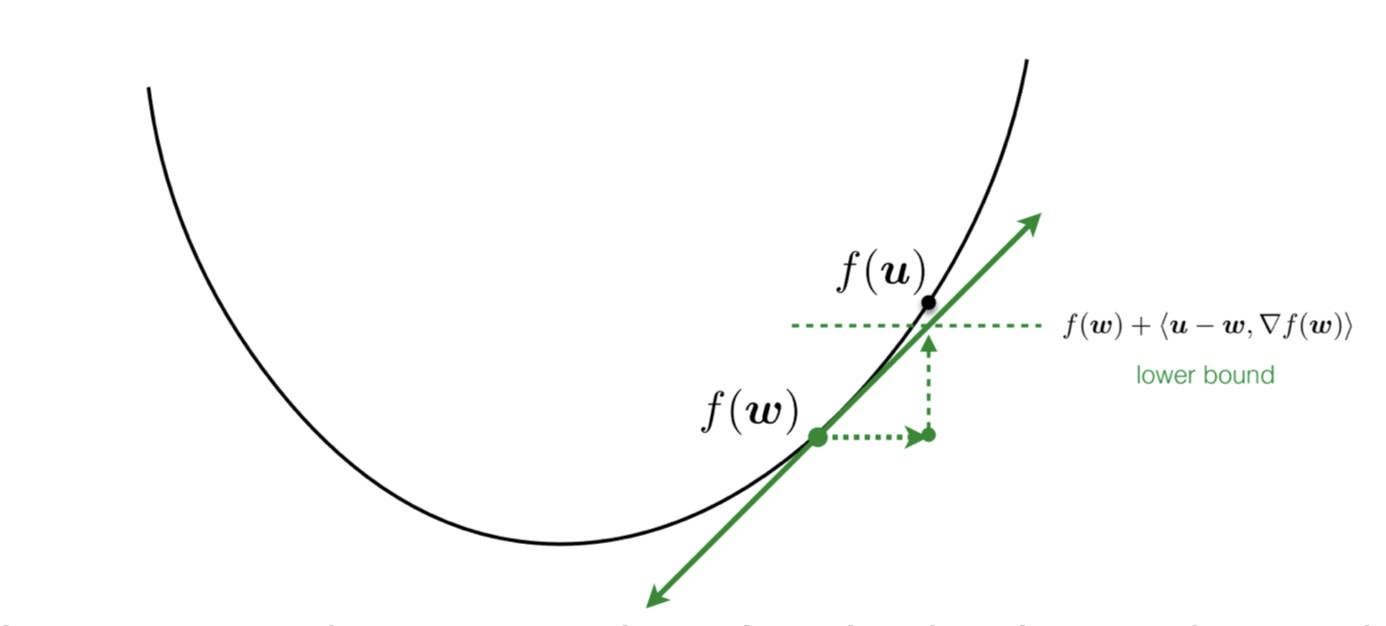
\includegraphics[scale=0.4]{images/gd_perspect2.png}
\end{center}


As $f(\textbf{u}) \approx f(\textbf{w}) + \langle (\textbf{u} - \textbf{w}), \nabla f(\textbf{w}) \rangle$ only holds when $\textbf{u}$ is close to $\textbf{w}$, we can add an L2 regularization term. 
$$\min_\textbf{u} \|\textbf{u}  - \textbf{w}\|_2^2$$
The full objective to minimize becomes
$$\min_\textbf{u} \frac{1}{2}\|\textbf{u}  - \textbf{w}\|_2^2 + \eta(f(\textbf{w}) + \langle (\textbf{u} - \textbf{w}), \nabla f(\textbf{w}) \rangle)$$
With switching the notation $\textbf{u} \rightarrow \textbf{w}$ and $\textbf{w} \rightarrow \textbf{w}^{(t)}$, the equation becomes
$$\textbf{w}^{(t+1)} = \text{argmin}_{\textbf{w}}\frac{1}{2}\|\textbf{w}  - \textbf{w}^{(t)}\|_2^2 + \eta(f(\textbf{w}^{(t)}) + \langle (\textbf{w} - \textbf{w}^{(t)}), \nabla f(\textbf{w}^{(t)}) \rangle)$$

Be taking the first order derivative to find the optimal $\textbf{w}$, we got the GD algorithm update rules.
$$\frac{\partial \frac{1}{2}\|\textbf{w}  - \textbf{w}^{(t)}\|_2^2 + \eta(f(\textbf{w}^{(t)}) + \langle (\textbf{w} - \textbf{w}^{(t)}), \nabla f(\textbf{w}^{(t)}) \rangle)}{\partial \textbf{w}} = 0$$
$$(\textbf{w}  - \textbf{w}^{(t)}) + \eta(0 + \nabla f(\textbf{w}^{(t)}) = 0$$
$$\textbf{w}^{(t+1)} = \textbf{w}^{(t)} - \eta \nabla f(\textbf{w}^{(t)})$$

\textbf{Isometric Quadratic Approximation  }
The third perspective is to approximate the function value using isometric quadratic approximation. Start with second order Taylor expansion
$$\min_u f(\textbf{u}) \approx \min_u \{f(\textbf{w}) + (\textbf{u} - \textbf{w})^T\nabla f(\textbf{w}) + \frac{1}{2}(\textbf{u} - \textbf{w})^T\nabla^2 f(\textbf{w})(\textbf{u} - \textbf{w})\}$$

\begin{center}
    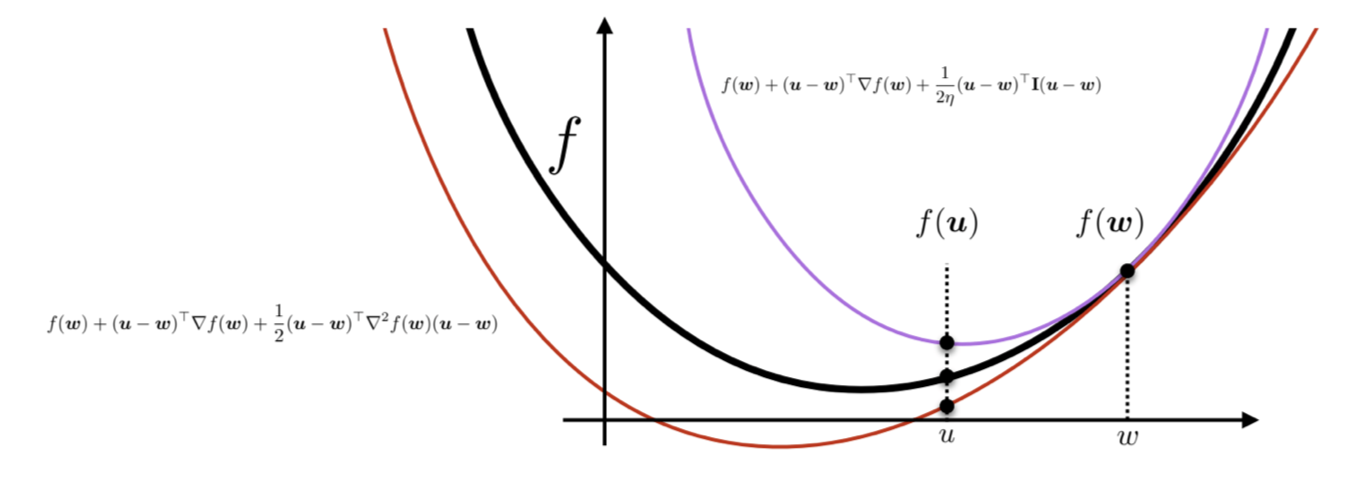
\includegraphics[scale=0.4]{images/gd_perspect3.png}
\end{center}

Using isometric quadratic approximation,
$$\min_u f(\textbf{u}) \approx \min_u \{f(\textbf{w}) + (\textbf{u} - \textbf{w})^T\nabla f(\textbf{w}) + \frac{1}{2\eta}(\textbf{u} - \textbf{w})^T\textbf{I}(\textbf{u} - \textbf{w})\}$$
where $\eta$ is a tunable variance parameter. \\
By multiplying the RHS objective function with $\eta$ and rearranging terms, the objective function becomes
$$\min_u \frac{1}{2}(\|\textbf{u} - \textbf{w})\|_2^2 + \eta(f(\textbf{w}) + (\textbf{u} - \textbf{w})^T\nabla f(\textbf{w}))$$
By similar manner with the linear approximation perspective, replacing the notation $\textbf{u} \rightarrow \textbf{w}$ and $\textbf{w} \rightarrow \textbf{w}^{(t)}$, we have
$$\textbf{w}^{(t+1)} = \text{argmin}_{\textbf{w}}\frac{1}{2}\|\textbf{w}  - \textbf{w}^{(t)}\|_2^2 + \eta(f(\textbf{w}^{(t)}) + \langle (\textbf{w} - \textbf{w}^{(t)}), \nabla f(\textbf{w}^{(t)}) \rangle)$$

The remaining step is taking the first order derivative to find minimum solution, which is exactly the same as the final step of linear quadratic approximation.

\subsubsection{Stochastic Gradient Descent}
From last subsection, we know that the update rule of gradient descent is 
$$\textbf{w}^{(t+1)} = \textbf{w}^{(t)} - \eta \nabla f(\textbf{w}^{(t)})$$

Most of the time calculating gradient $\nabla f(\textbf{w})}$  requires summing over all data points, which may not be feasible when dataset size is large. To speed up, one can replace the gradient by randomly sampled data points instead of exact gradient at each iteration; that leads to Stochastic Gradient Descent \cite{Robbins2007ASA}, listed as Algorithm \ref{algo:sgd}. 
\begin{algorithm}[H]
\caption{Stochastic Gradient Descent (SGD)}
\label{algo:sgd}
\begin{algorithmic}[1]
\STATE $\textbf{w}^{(0)} \leftarrow 0$ \hfill $\triangleright$ Weight initialization
\STATE $\eta > 0$
\FOR{$t=1,\;\cdots,\;T$}
\STATE $z \sim \mathcal{D}$ \hfill $\triangleright$ Sampled mini-batch z from full dataset
\STATE $\textbf{v}^{(t)} = \nabla_z f(\textbf{w}^{(t-1)})$ \hfill $\triangleright$ Compute gradient from sampled data instead of full data points
\STATE $\textbf{w}^{(t)} = \textbf{w}^{(t-1)} - \eta \textbf{v}^{(t)})$ \hfill $\triangleright$ Update weight with $\textbf{v}^{(t)}$ instead of exact gradient
\ENDFOR
\end{algorithmic}
\end{algorithm}

Different from GD, SGD sampled the mini-batch for calculating gradient at line 3. The gradient for update is calculated through sampled mini-batch at line 4 and is used for update at line 5. With such sampling, we can reduce the computation on gradient while remaining the expected value of gradient being the same as exact gradient at each iteration. One key observation of SGD is that the algorithm does not require the access of full dataset at each iteration, which looks like online convex optimization.

\subsubsection{Online Gradient Descent(OGD) as Online Mirrow Descent (OMD)}

We started from showing that the Online Gradient Descent algorithm is actually Online Mirrow Descent with linear loss and quadratic regularizer. Starting from defining the regularization function

$$\psi (\textbf{w}) = \frac{1}{2\eta} \| \textbf{w} \|_2^2$$

And the loss function

$$f(w) = \langle \textbf{w}, \theta \rangle $$


Our update rule becomes 

$$\textbf{w}^{(t+1)} =  \text{argmin}_{\textbf{w}} \langle \textbf{w}, - \theta^{(t+1)}\rangle + \frac{1}{2\eta} \| w \|_2^2$$

By solving the first order partial derivative equals to 0, we can find the minimizer
$$\textbf{w}^{(t+1)} = -\eta \theta$$
which is the mirror function. \\
Algorithm \ref{algo:osgd} is the Online Sub-Gradient Descent, which adapted the OMD algorithm with the mirror function induced from linear loss function and quadratic regularizer.
\begin{algorithm}[H]
\caption{Online Sub-Gradient Descent}
\label{algo:osgd}
\begin{algorithmic}[1]
\FOR{$t=1,\;\cdots,\;T$}
\STATE $\theta^{(t+1)} = \theta^{(t)} - \eta \textbf{z}$ \hfill $\triangleright$ $ \textbf{z}^{(t)} = \partial f^{(t)}(\textbf{w}^{(t)})$
\STATE $\textbf{w}^{(t+1)} = -\eta \theta^{(t+1)}$ \hfill $\triangleright$ Mirror Projection
\ENDFOR
\end{algorithmic}
\end{algorithm}
From line 2 and 3 of Algorithm \ref{algo:osgd}, we can further show that it is same ass GD update rule by 
$$\textbf{w}^{(t+1)} = -\eta \theta^{(t+1)}$$
$$= -\eta \sum_{i=1}^t \textbf{z}^{(i)}$$
$$= -\eta (\textbf{z}^{(t)} + \theta ^{(t)})$$
$$= -\eta (\textbf{z}^{(t)} - \frac{1}{\eta}\textbf{w} ^{(t)})$$
$$= \textbf{w}^{(t)} - \eta \textbf{z}^{(t)}$$

Algorithm \ref{algo:opsgd} is the Online Projected Sub-Gradient Descent, with mirror function also projecting dual parameter $\theta$ to some conditioned set. 
\begin{algorithm}[H]
\caption{Online Projected Sub-Gradient Descent}
\label{algo:opsgd}
\begin{algorithmic}[1]
\FOR{$t=1,\;\cdots,\;T$}
\STATE $\theta^{(t+1)} = \theta^{(t)} - \eta \textbf{z}$ \hfill $\triangleright$ $ \textbf{z}^{(t)} = \partial f^{(t)}(\textbf{w}^{(t)})$
\STATE $\textbf{w}^{(t+1)} = \Pi_{\theta \rightarrow S}-\eta \theta^{(t+1)}$ \hfill $\triangleright$ Mirror Projection
\ENDFOR
\end{algorithmic}
\end{algorithm}

\subsubsection{Analysis of Online Gradient Descent}
To analyze the regret bound, we first use the general regret bound from OMD

$$
R(\textbf{u}) \leq \psi (\textbf{u}) - \psi (\textbf{w}^{(1)}) + \sum_{t=1}^T D_{\psi^*} (\mathbf{\theta^{(t+1)}} \| \mathbf{\theta^{(t)}})
$$

As our regularizer is defined as 
$$\psi (\textbf{w}) = \frac{1}{2} \| \textbf{w} \|_2^2$$
its convex conjugate $\psi^*$ is also L2 norm. Combining with the definition of Bregman divergence $D_{\psi^*} (\mathbf{\theta^{(t+1)}} \| \mathbf{\theta^{(t)}}) = \psi^* (\mathbf{\theta}^{(t+1)}) - \psi^* (\mathbf{\theta}^{(t)}) - \nabla \psi^* (\mathbf{\theta}^{(t)})(\mathbf{\theta}^{(t+1)} - \mathbf{\theta}^{(t)})$. Thus the RHS of OMD regret bound will become
$$
R(\textbf{u}) \leq \frac{1}{2\eta} \| \textbf{u} \|_2^2 - \frac{1}{2\eta}\| \textbf{w}^{(1)} \|_2^2 + \sum_{t=1}^T \frac{1}{2\eta}\|\mathbf{\theta}^{(t+1)} \|_2^2 - \frac{1}{2\eta}\|\mathbf{\theta}^{(t)}\|_2^2 - \frac{1}{2\eta}\nabla \|\mathbf{\theta}^{(t)}\|_2^2(\mathbf{\theta}^{(t+1)} - \mathbf{\theta}^{(t)})
$$

$$
= \frac{1}{2\eta} \| \textbf{u} \|_2^2 - \frac{1}{2\eta}\| \textbf{w}^{(1)} \|_2^2 + \sum_{t=1}^T \frac{1}{2\eta}\|\mathbf{\theta}^{(t+1)} \|_2^2 + \frac{1}{2\eta}\|\mathbf{\theta}^{(t)}\|_2^2 - \frac{1}{\eta} \mathbf{\theta}^{(t)}\mathbf{\theta}^{(t+1)}
$$

By completing the square for the summation term
$$
R(\textbf{u}) \leq \frac{1}{2\eta} \| \textbf{u} \|_2^2 - \frac{1}{2\eta}\| \textbf{w}^{(1)} \|_2^2 + \sum_{t=1}^T \frac{1}{2\eta} \|\mathbf{\theta}^{(t+1)} - \mathbf{\theta}^{(t)} \|_2^2
$$

$$
= \frac{1}{2\eta} \| \textbf{u} \|_2^2 - \frac{1}{2\eta}\| \textbf{w}^{(1)} \|_2^2 + \sum_{t=1}^T \frac{1}{2\eta} \|\mathbf{\theta}^{(t)} - \eta \textbf{z}^{(t)} -  \mathbf{\theta}^{(t)} \|_2^2
$$

$$
\leq \frac{1}{2\eta} \| \textbf{u} \|_2^2  + \sum_{t=1}^T \frac{\eta}{2} \|\textbf{z}^{(t)} \|_2^2
$$
By setting up the maximum range of primal space parameter D and maximum gradient size G

$$D = \max_u \| u \|_2 \textbf{   } u \in S$$
$$G = \max_z \| z \|_2 \textbf{   } z \in \partial f(\textbf{w})$$
the above bound becomes
$$R(\textbf{u}) \leq \frac{D^2}{2\eta}   + T\frac{\eta}{2}G^2$$
To minimize the RHS, we can pick optimal $\eta$ by setting the parital derivative w.r.t. $\eta$ equals 0.
$$\frac{\partial \frac{D^2}{2\eta}   + T\frac{\eta}{2}G^2}{\partial \eta}$$

$$= \frac{-D^2}{2\eta^2}   + \frac{TG^2}{2}=0$$
$$\eta = \frac{D}{G\sqrt{T}}$$
Plug in back to the original equation
$$R(\textbf{u}) \leq GD\sqrt{T}$$
% \subsection{Randomized Weighted Majority Algorithm (RWMA)}

% Now, we introduce the Randomized Weighted majority Algorithm (RWMA), listed as Algorithm \ref{algo:rwma} below. It is known by many different names, such as Exponentiated Weighted Majority, Hedge Algorithm etc. The key difference from WMA is that we create a multinomial distribution using the weights and make the learner prediction via sampling from this distribution (Line 5, 6).

% \begin{algorithm}[H]
% \caption{Randomized Weighted Majority Algorithm (RWMA)}
% \label{algo:rwma}
% \begin{algorithmic}[1]
% \STATE $\textbf{w}^{(1)} \leftarrow \{w_n^{(1)}=1\}_{n=1}^N$ \hfill $\triangleright$ Weight initialization
% \STATE $\eta\leq\frac{1}{2}$\hfill $\triangleright$ Penalty rate initialization
% \FOR{$t=1,\;\cdots,\;T$}
% \STATE \textsc{Receive} ($\textbf{x}^{(t)}\in\{-1, 1\}^N$) \hfill $\triangleright$ Receive experts predictions
% \STATE $I\sim$ \textsc{Multinomial}($\textbf{w}^{(t)}/\Phi^{(t)}$), where $\Phi^{(t)}=\sum_{n=1}^Nw_n^{(t)}$
% \STATE $\hat{y}^{(t)}=h_i(\textbf{x}^{(t)})$ \hfill $\triangleright$ Make learner prediction via sampling
% \STATE \textsc{Receive} ($y^{(t)}\in\{-1, 1\}$) \hfill $\triangleright$ Receive actual answer
% \STATE $w_n^{(t+1)}\leftarrow w_n^{(t)}\big(1-\eta\cdot\textbf{1}[y^{(t)}\neq h_n(\textbf{x})^{(t)}]\big)$ \hfill $\triangleright$ Weight update
% \ENDFOR
% \end{algorithmic}
% \end{algorithm}

% Now, let's derive the mistake bound for RWMA. We will find that the expected number of mistakes for RWMA is upper bounded and the mistake bound is better than a factor of 2, when compared to the WMA. But first, we state a simple lemma to help derive further results in Theorem 9.


% \lemma{$e^x\geq 1+ x$ for all $x\in\mathbb{R}$.}\label{lemma:2}
% \proof{One can easily show the above inequality by applying Taylor expansion to $e^x$.}
% \theorem{(Mistake bound of RWMA) Let $M^{(t)}, m_i^{(t)}$ respectively be the number of mistakes that have been made by the RWMA learner and the $i$-th hypothesis until the time step $t$, and $N, \eta$ be the number of experts and the penalty rate. Then, expected mistakes of learner $\mathbb{E}[M^{(t)}]$ is upper-bounded as:
% $$\mathbb{E}[M^{(t)}]\leq (1+\eta)m_i^{(t)} + \frac{\log{N}}{\eta}$$}\label{theorm:rwma}
% \proof{Lets again define the potential function $\Phi^{(t)}$ for RWMA as the sum of weights:
% \begin{align}
%   \Phi^{(t)} = \sum_{n=1}^N w_n^{(t)}\label{eq:rwma_potential}
% \end{align}
% By the weight update rule of RWMA, $w_n^{(t+1)}$ can be analytically calculated from $w_n^{(t)}$ as follows:
% \begin{align}
%     w_n^{(t+1)}= \big(1-\eta\cdot\textbf{1}[y^{(t)}\neq y_n^{(t)}]\big)w_n^{(t)}=\big(1-\eta\alpha_n^{(t)}\big)w_n^{(t)}\;\;\;\;\;(\text{where} \;\alpha_n^{(t)}=\textbf{1}[y^{(t)})\neq y_n^{(t)}]\label{eq:rwma_weight}
% \end{align}
% By combining Eq. (\ref{eq:rwma_weight}) \& (\ref{eq:rwma_potential}), one can derive the mathematical relation between $\Phi^{(t+1)}$ and $\Phi^{(t)}$ as follows:
% \begin{align}
%     \Phi^{(t+1)}=\sum_n w_n^{(t+1)}&=\sum_n (1-\eta\alpha_n^{(t)})w_n^{(t)}\;\;\;(\because \text{Eq.}\; (\ref{eq:rwma_weight}))\nonumber\\
%     &=\sum_n w_n^{(t)} - \sum_n \eta\alpha_n^{(t)}w_n^{(t)}\nonumber\\
%     &=\Phi^{(t)} - \frac{\Phi^{(t)}}{\Phi^{(t)}}\sum_n \eta\alpha_n^{(t)}w_n^{(t)}\nonumber\\
%     &=\Phi^{(t)} - \Phi^{(t)}\eta\sum_n \alpha_n^{(t)}\frac{w_n^{(t)}}{\Phi^{(t)}}\nonumber\\
%     &=\Phi^{(t)} - \Phi^{(t)}\eta\sum_n \alpha_n^{(t)}p_n^{(t)}\;\;\;(\text{where}\;p_n^{(t)}=\frac{w_n^{(t)}}{\Phi^{(t)}})\nonumber\\
%     &=\Phi^{(t)}\Big(1-\eta\sum_n\alpha_n^{(t)}p_n^{(t)}\Big)\label{eq:rwma_abc}
% \end{align}
% Assuming all weights are initialized to 1, $\Phi^{(T+1)}$ can be calculated by recursively applying Eq. ({\ref{eq:rwma_abc}}) as follows:
% \begin{align}
%     \Phi^{(T+1)}=\Phi^{(1)}\prod_{t=1}^{T}\Big(1-\eta\sum_n\alpha_n^{(t)}p_n^{(t)}\Big)=N\prod_{t=1}^{T}\Big(1-\eta\sum_n\alpha_n^{(t)}p_n^{(t)}\Big)\label{eq:rwma_xyz}
% \end{align}
% We can now derive the upper bound of $\Phi^{(T+1)}$ by combining Lemma \ref{lemma:2} and Eq. (\ref{eq:rwma_xyz}) as follows:
% \begin{align}
%     \Phi^{(T+1)}&=N\prod_{t=1}^{T}\Big(1-\eta\sum_n\alpha_n^{(t)}p_n^{(t)}\Big)\nonumber\\
%     &\leq N\prod_{t=1}^T\exp{\Big(-\eta\sum_n\alpha_n^{(t)}p_n^{(t)}\Big)}\;\;\;(\because \text{Lemma}\;\ref{lemma:2})\nonumber\\
%     &=N\exp{\Big(-\eta\sum_{t=1}^{T}\mathbb{E}\big[\textbf{1}[y^{(t)}\neq\hat{y}^{(t)}]\big]\Big)}\;\;\;(\because\;\sum_n\alpha_n^{(t)}p_n^{(t)}=\mathbb{E}_p\big[\textbf{1}[y^{(t)}\neq\hat{y}^{(t)}]\big])\nonumber\\
%     &=N\exp{\big(-\mathbb{E}[M^{(T)}]\big)}\;\;\;(\because\;\text{definition of}\;M^{(t)})\label{eq:rwma_upper}
% \end{align}
% By applying the same argument as in WMA, the lower bound of $\Phi^{(T+1)}$ is $(1-\eta)^{m_n^{(T)}}$.
% \begin{align}
%     \Phi^{(T+1)}\geq(1-\eta)^{m_n^{(T)}}\label{eq:rwma_lower}
% \end{align}
% By combining Eq. (\ref{eq:rwma_upper}) \& (\ref{eq:rwma_lower}), we can now derive the mathematical relation between $\mathbb{E}[M^{(t)}]$ and $m_n^{(t)}$ as follows:
% \begin{align}
%     (1-\eta)^{m_n^{(T)}}\leq \Phi^{(T+1)} \leq N\exp{\big(-\mathbb{E}[M^{(T)}]\big)}\label{eq:rwma_init}
% \end{align}
% Finally, we can compute the (upper) bound of expected mistakes $\mathbb{E}[M^{(t)}]$ by combining the bounds of $\Phi^{(t+1)}$ (Eq. (\ref{eq:rwma_init})) and Lemma \ref{lemma:1} as follows:
% \begin{align*}
%     m_n^{(T)}\log(1-\eta) &\leq \log N - \eta\mathbb{E}[M^{(T)}]\\
%     m_n^{(T)}(-\eta-\eta^2)&\leq \log N - \eta\mathbb{E}[M^{(T)}] \;\;\;(\because\; \text{Lemma}\;\ref{lemma:1})\\
%     -m_n^{(T)}(1+\eta)&\leq\frac{\log N}{\eta} - \mathbb{E}[M^{(T)}]\\
%     \mathbb{E}[M^{(T)}]&\leq (1+\eta)m_n^{(T)} + \frac{\log N}{\eta}
% \end{align*}
% Therefore, we have obtained the upper bound of expected regret for RWMA.\QED
% }

% We are now interested in the performance (regret bound) of RWMA algorithm.
% \theorem{RWMA is a no-regret algorithm.}
% \proof{By the definition of regret and Theorem \ref{theorm:rwma}}, we could obtain the upper bound of \textit{expected regret} of RWMA, $\mathbb{E}[R]$, as follows:
% \begin{align}
%     \mathbb{E}[R] = \mathbb{E}[M^{(T)}] - m_n^{(T)} \leq \eta m_n^{(T)} + \frac{\log N}{\eta} \label{eq:rwma_final}
% \end{align}
% If we set $\eta$ to $\frac{1}{\sqrt{T}}$, both $\eta m_n^{(T)}$ and $\frac{\log N}{\eta}$ follow $O(\sqrt{T})$.\\
% Thus, $\frac{\mathbb{E}[R]}{T} = \Big(\eta m_n^{(T)} + \frac{\log N}{\eta}\Big) \propto \frac{1}{\sqrt{T}}\rightarrow 0\;\text{as}\;T\rightarrow\infty$.\QED

% \subsection{Online Linear Classification}

% Now we will start with an Online Linear Classification (OLC) algorithm. Here, we are moving from an exhaustive space to a sampled space, unlike the characterization in Section 1.1. Further, we don't want to program the behavior of the algorithm but learn from an expert, and we will start with two algorithms involving linear hyperplanes to learn the decision boundary:
% \begin{enumerate}
%     \item Perceptron algorithm, which has additive updates.
%     \item Winnow Algorithm, which has multiplicative updates.
% \end{enumerate}
% \begin{algorithm}[H]
% \caption{Perceptron algorithm}
% \label{algo:perceptron}
% \begin{algorithmic}[1]
% \STATE $\textbf{w}^{(1)} \leftarrow 0$ \hfill $\triangleright$ Weight initialization
% \FOR{$t=1,\;\cdots,\;T$}
% \STATE \textsc{Receive} ($\textbf{x}^{(t)}\in R^N$) \hfill $\triangleright$ Receive expert predictions
% \STATE $\hat{y}^{(t)} = \text{sign}\Big(w^{(t)} x^{(t)}\Big)$ \hfill $\triangleright$ Make learner prediction
% \STATE \textsc{Receive} ($y^{(t)}\in\{-1, 1\}$) \hfill $\triangleright$ Receive actual answer
% \STATE $w_n^{(t+1)}\leftarrow w_n^{(t)} + y^{(t)} \cdot x^{(t)} \cdot\textbf{1}[y^{(t)}\neq x_n^{(t)}] $ \hfill $\triangleright$ Weight update
% \ENDFOR
% \end{algorithmic}
% \end{algorithm}

% In the perceptron algorithm (listed as Algorithm \ref{algo:perceptron} above), if the prediction is correct then no updates are made. Further, we can ask the following questions to characterize the perceptron algorithm:

% \begin{enumerate}
%     \item Is the perceptron algorithm fast? Yes. No weight updates are done for correct prediction, while the incorrect prediction update just involves computing a simple dot product and a sum. The prediction itself is just a dot product.
%     \item Is it a Large Margin classifier? No, there is no notion of margin in the algorithm.
%     \item Does it work on non-separable data? No, but when the data is linearly separable, the perceptron algorithm will make a finite number of mistakes.
% \end{enumerate}

% Now again we could derive the mistake bound, following the similar 5-step strategy, as we had used with the weighted majority algorithms. We list the Perceptron Mistake Bound:

% \begin{align}
%     M \leq \frac{R^{2}}{\gamma^{2}}
% \end{align}

% Here, $R = \maximize_{t} \Vert x^{t}\Vert$ is the norm of the obserbvations and $\gamma = \minimize_{t} y_{t} $ is the margin of separability.

% Further, Block and Novikoff \cite{novikoff1963convergence} give the mistake bound, but not the regret bound because under the conditions of linear separability, we do not really need to consider regret, as described in Section 1.2.

\subsection{Online Normalized Exponentiated Gradient Descent}
If we define the regularization function and the loss function in OMD as:
$$
\psi(\bm{w}) = \sum_{k=1}^K  w_k \log w_k \;\;\; \bm{w} \in \mathbb{S}^K
$$
$$
f(\bm{w}) = \big\langle\bm{w}, \bm{\theta}\big\rangle
$$
We call this online normalized exponentiated gradient descent (ONEGD). Then the prediction rule becomes:
$$
\bm{w}^{(1+t)} = \argmin{\bm{w}\in\mathbb{S}^K} \big\langle \bm{w}, -\bm{\theta^{(t+1)}} \big\rangle + \sum_{k=1}^K w_k \log w_k
$$
Let's add the simplex constraint to objective and call the objective as Lagrangian:
$$
L = \big\langle \bm{w}, -\bm{\theta^{(t+1)}} \big\rangle + \frac{1}{\eta}\sum_{k=1}^K w_k \log w_k + \lambda(1-\sum_k w_k) 
$$
We do first derivative to find the minimizer for linear loss and entropic regularization.
$$
\frac{\partial L}{\partial w_k} = -\theta_k + \frac{1}{\eta} (1+\log w_k) - \lambda
$$
$$
0 = -\theta_k + \frac{1}{\eta} + \frac{1}{\eta}\log w_k - \lambda
$$
$$
\rightarrow w_n = \frac{\exp(\eta\theta_k)}{\exp(1-\eta\lambda)}
$$
The dual parameter update is as below.
$$
\theta^{(t+1)} = \theta^{(t)} - \eta\bm{z}^{(t)}, \bm{z}^{(t)} \in \partial f^{(t)}(\bm{w}^{(t)})
$$
Since mirror function enforces the geometry of the problem, the mirror function becomes
$$
g(\bm{\theta}) = \frac{\exp(\eta\bm{\theta})}{\sum_{n'}\exp \eta\theta_{n^'}}
$$



Algorithm of ONEGD is shown in Algorithm \ref{algo:onegd}
\begin{algorithm}[H]
\caption{Online Norm-Exp-GD}
\label{algo:onegd}
\begin{algorithmic}[1]
\FOR{$t=1,\;\cdots,\;T$}
\STATE $\theta^{(t+1)} = \theta^{(t)} - \eta \textbf{z}$, $ \textbf{z}^{(t)} = \partial f^{(t)}(\textbf{w}^{(t)})$ \hfill Dual Parameter Update
\STATE $\textbf{w}^{(t+1)} = \Pi_{\theta \rightarrow S}-\eta \theta^{(t+1)}$ \hfill $\triangleright$ Mirror Projection
\ENDFOR
\end{algorithmic}
\end{algorithm}

It is worth noting that the update of ONEGD is the same update as the weighted majority algorithm. We can have this conclusion from
$$
w_n^{(t+1)} = \frac{\exp(\eta \theta_n^{(t+1)})}{\sum_{n'}\exp(\theta_{n'})}
$$
$$
=\frac{w_n^{(t)}\exp(-\eta z_n^{(t)})}{\sum_k w_k^{(t)}\exp(-\eta z_n^{(t)})}
$$
$$
\rightarrow w_n^{(t+1)} \propto w_n^{(t)}\exp(-\eta z_n^{(t)})
$$

Lastly, we show Hedge algorithm in Algorithm \ref{algo:hedge}, which is an unnormalized exponentiated gradient descent algorithm.
\begin{algorithm}[H]
\caption{Hedge Algorithm (\beta)}
\label{algo:hedge}
\begin{algorithmic}[1]
\STATE $\textbf{w}^{(1)}$ $\leftarrow \{w_n^{(1)} = 1\}_{n=1}^N$ \hfill $\triangleright$ Weight initialization
\FOR{$t=1,\;\cdots,\;T$}
\STATE \textsc{Receive} $(\bm{x}^(t) \in \{-1, 1\})$ \hfill
\STATE $i \sim \textsc{Multinomial}(\bm{w}^{(t)}/\Phi^{(t)})$ \hfill
\STATE $\hat{y} = h_i(\bm{x}^{(t)})$ \hfill $\triangleright$ Expeceted 0-1 loss is a linear loss
\STATE \textsc{Receive} $y^t \in \{-1, 1\}$ \hfill
\STATE $w_n^{(t+1)} = w_n^{(t)}e^{-\beta (\bm{1}[y^{(t)} \neq h_n(\bm{x}^{(t)})])}$ \hfill $\triangleright$ Exponential update comed from entropic regularization
\ENDFOR
\end{algorithmic}
\end{algorithm}


%\section*{References}
%Include your references here. Please cite any resources you found useful.	
%Populate the refs.bib file or list your references manually. Be consistent in formatting!
{
\bibliography{refs}
\bibliographystyle{abbrv}
}

%\section{Appendix}
%This section provides any relevant background material that was not covered in the lectures, but was found to be useful for understanding the material. 
%For example, derivations, theory underlying techniques employed, etc. 

%Additionally, this section can summarizes applications or extensions of these techniques found in the literature. 

\end{document} % Done!


